%class
	\documentclass{beamer}

%template
	\usetheme{HannoverSalman}
	\setbeamertemplate{navigation symbols}{}
	%\setbeamertemplate{footline}{\centering{\insertframenumber/\insertpresentationendpage}}
	%\setbeamertemplate{footline}{\hspace*{.5cm}\scriptsize{\hfill\insertframenumber\hspace*{.5cm}}} 


%packages
	\usepackage{amsmath, amssymb, graphicx,cancel}
	\usepackage[absolute,overlay]{textpos}
	\usepackage{subfigure}
	\usepackage{caption}\captionsetup{labelformat=empty,labelsep=none}
	\usepackage{geometry}
	\geometry{verbose}
	\usepackage{color}
	\usepackage{xmpmulti}
	\usepackage[3D]{movie15}
	\usepackage{hyperref}
%	\usepackage{bookmark}
	\usepackage[open,openlevel=4,atend]{bookmark}
	%\bookmarksetup{color=blue}
	\usepackage{multirow}
	\usepackage[style=numeric,defernumbers, authoryear]{biblatex}
	%\usepackage[square,sort]{natbib}
	%\usepackage{fancyhdr}%\pagestyle{fancy} 

	
	\hypersetup{bookmarksdepth = 4}


%citations files
	\bibliography{MyCitations}

%logoCSIPCPL
    \setlength{\TPHorizModule}{1mm}
    \setlength{\TPVertModule}{1mm}
    \newcommand{\logoCSIPCPL}
    {
    	\begin{textblock}{1}(100,2) %(100,85)  for bottom
    		
\includegraphics[width=1.5cm]{figs/logo_CSIP}
    	\end{textblock}
    	
	\begin{textblock}{1}(117,1) %(117,85)  for bottom
    		
\includegraphics[width=1.0cm]{figs/logo_CPL}
    	\end{textblock} 
    }

%logo evolution
    \newcommand{\logoEvolution}
    {    	
	\begin{textblock}{1}(110,1) %(117,85)  for bottom
    		\includegraphics[width=0.65in]{figs/logo_evolution.pdf}
    	\end{textblock} 
    }

%logo Qualcomm
    \newcommand{\logoQualcomm}
    {
    	\begin{textblock}{1}(110,2) %(100,85)  for bottom
    		\includegraphics[width=1.5cm]{figs/logo_qualcomm.jpg}
    	\end{textblock}
    }
%logo Qualcomm (long)
    \newcommand{\logoQualcommllong}
    {
    	\begin{textblock}{1}(0,0) 
    		\includegraphics[width=1.25in]{figs/logo_qualcomm_long.jpg}
    	\end{textblock}
    }

%logo Tech Tower
    \newcommand{\logoTechTower}
    {
    	\begin{textblock}{1}(0,0) 
    		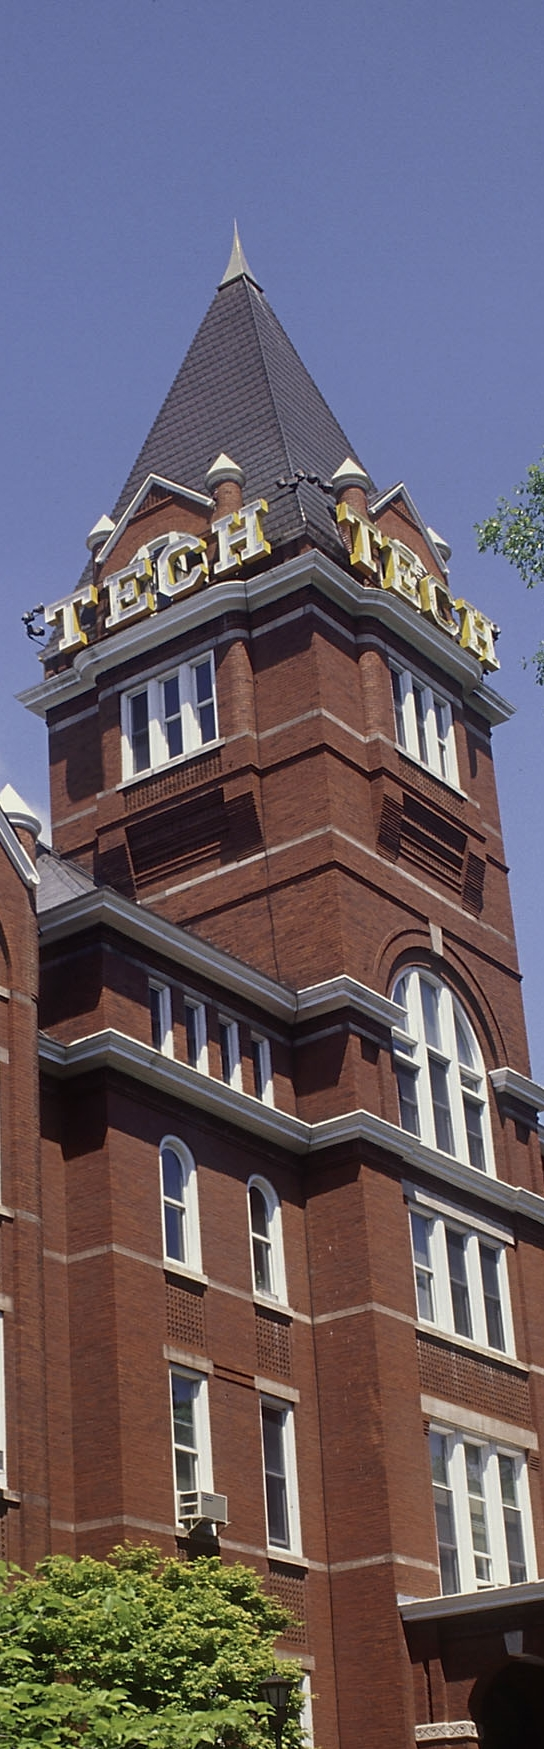
\includegraphics[width=1.25in]{figs/logo_TechTower.jpg}
    	\end{textblock}
    }

%logo tree
    \newcommand{\logoTree}
    {
    	\begin{textblock}{1}(0,0) 
    		\includegraphics[width=1.25in]{figs/logo_tree.jpg}
    	\end{textblock}
    }
%page numbers
    \newcommand{\mypagenum}
    {
    	\begin{textblock}{1}(1,94) 
		{\tiny \color[rgb]{0.2,0.2,1}\insertframenumber} %\insertframenumber,\insertpresentationendpage, \inserttotalframenumber
    	\end{textblock}
    }
%my footnote citation
	\newcommand{\myFootnoteCitation}[2]
	{
		\footnote{\tiny \citeauthor{#1}, \emph{#2}, \citeyear{#1}.}  %\citeauthor{#1}, \citetitle{#1}, #2 \citeyear{#1}.
	}
%my refer to citation
	\newcommand{\mycite}[1]
	{
		\emph{\citeauthor{#1} (\citeyear{#1})}
	}
%my footnote website citation
	\newcommand{\myFootnoteWebsiteCitation}[1]
	{
		\footnote{\tiny \citeauthor{#1}}
	}

\let\thefootnote\relax\footnotetext{Footnotetext without footnote mark}


%section underline
%\newcommand{\tmpsection}[1]{}
%\let\tmpsection=\section
%\renewcommand{\section}[1]{\tmpsection{\underline{#1}}}



%commands
	\newcommand{\likelihood}{p(Z_k| x_k) }						%likelihood
	\newcommand{\prior}{p(x_k)  } 								%prior
	\newcommand{\posterior} {p(x_k| Z_k)}						%posterior
	\newcommand{\prediction} {p(x_k| Z_{k-1})}					%prediction
	\newcommand{\update} {p(x_k|Z_k)}							%update
	\newcommand{\observations} {p(Z_k)}						%observations
	\newcommand{\prevobservations} {p(Z_{k-1})}				%previous observations
	\newcommand{\dxpk} {dx_{k-1}}							%dx_{k-1}
	\newcommand{\ChapKolm}{\int{p(x_k| x_{k-1})p(x_{k-1}|Z_{k-1})} \dxpk} %Chapman Kolmogorov

	%algorithm specific: JPDAF
	\newcommand{\likelihoodJPDAF}{p(Z_k| \chi, m, Z_{k-1}) }		%1. likelihood
	\newcommand{\priorJPDAF}{p(\chi|m, Z^{k-1}} 				%2. prior	
	\newcommand{\observationsJPDAF} {p(Z_k}					%3. observations
	\newcommand{\posteriorJPDAF} {p(\chi| Z_k)}					%4. posterior

%environments
	\newenvironment{changemargin}[2]
	{
	  	\begin{list}{}
		{
			\setlength{\topsep}{0pt}%
			\setlength{\leftmargin}{#1}%
			\setlength{\rightmargin}{#2}%
			\setlength{\listparindent}{\parindent}%
			\setlength{\itemindent}{\parindent}%
			\setlength{\parsep}{\parskip}%
		}
	  	\item[]
		}
		{\end{list}
	}
%figures

%colors
\definecolor{darkgreen}{rgb}{0,0.5,0}

%personal details
	\author{Salman Aslam}
	\institute{Advisor, Dr Christopher Barnes (ECE)\\Co-advisor, Dr Aaron Bobick (CoC)\\Georgia Institute of Technology}
	\date{}

\begin{document}
%####################################################################################################
\title{Visual Tracking \\ (experiments)}
%####################################################################################################
\begin{frame}[plain]\logoTechTower
	\titlepage
\end{frame}

\begin{frame}
\frametitle{Outline}
\logoCSIPCPL\logoTechTower
	\setcounter{tocdepth}{1}	
	\tableofcontents
\end{frame}

%#######################################################################
\section{INTRODUCTION}
%#######################################################################


%#######################################################################
\section{METHODOLOGY}
%#######################################################################
%\begin{frame}[plain]
%\frametitle{Experiments}
%\framesubtitle{classification and action recognition}
%\mypagenum
%	\begin{changemargin}{-1.35in}{0in}
%		\begin{figure}
%			\includegraphics[width=1.35\textwidth]{figs/format_classification_actionRecognition.pdf}
%		\end{figure}
%	\end{changemargin}
%\end{frame}









\begin{frame}
\frametitle{Methodology}
\framesubtitle{Image error metrics}
\mypagenum
	\begin{figure}
		\includegraphics[height=0.85\textheight]{figs/SP_imageMetrics.pdf}
	\end{figure}
\end{frame}


\begin{frame}
\frametitle{Methodology}
\framesubtitle{RVQ steps: static codebooks}
\mypagenum
	\begin{enumerate}\tiny
		\item {\color{red} 5 min:} create .raw files for say 6 or 7 images, go to the SQLScripts folder and put an entry for these images in say ECE8833a\_ImageDat.sql, and run it in Microsoft SQL Server
		\item {\color{red} 5 min:} open a .raw file in Snipper and select training snippets from this .raw file, also save file with overlaid snippets
		\item {\color{red} 5 min:} export these snippets from Microsoft SQL Server using Import and Export Data (32-bit) to .rpt file and change to .csv in Excel
		\item {\color{red} 5 min:} in Matlab, run RVQ\_sml to create .sml input file
		\item {\color{red} 5 min:} in Matlab, run gen to .ecbk, .dcbk, .stat, .idx training files
		\item {\color{red} 5 min:} in Matlab, run explorer to create .cor, .stg, .idx for first testing file
		\item {\color{red} ? min:} repeat for all testing files		
		\item {\color{red} 5 min:} create inner image
		\item {\color{red} 5 min:} create 2D image of .cor, .stg files
		\item {\color{red} 5 min:} create 3D image of .cor, .stg files
	\end{enumerate}
\end{frame}




%#######################################################################
\section{EXPERIMENTS}
%#######################################################################
%==============================================
\subsection{\ \ \ \ overview}
%==============================================
\begin{frame}
\frametitle{Experiments}
\framesubtitle{overview}
\mypagenum
	%\begin{changemargin}{-1.35in}{0in}
		\begin{figure}
			\includegraphics[width=1.0\textwidth]{figs/PhD_experimentalPlan.pdf}
		\end{figure}
	%\end{changemargin}
\end{frame}



\begin{frame}[plain]
\frametitle{EXPERIMENTS}
\framesubtitle{RVQ tracker}
\mypagenum
	\begin{changemargin}{-1.35in}{0in}
		\begin{figure}
			\includegraphics[width=1.35\textwidth]{figs/RVQ_tracker.pdf}
		\end{figure}
	\end{changemargin}
\end{frame}

%#######################################################################
\section{EXPERIMENTS (GT1)}
%#######################################################################


%==============================================
\subsection{\ \ \ \ single target, static codebooks}
%==============================================


\begin{frame}
\frametitle{\small EXPERIMENTS, GT1 (single target, static codebooks)}
\framesubtitle{overview}
\mypagenum
	\begin{itemize}
		\item simple one image, single target experiment to see how RVQ compares with template matching in detecting targets from the very image on which it was trained
	\end{itemize}
\end{frame}



\begin{frame}
\frametitle{\small EXPERIMENTS, GT1 (single target, static codebooks)}
\framesubtitle{overview (cont.)}
\mypagenum
	\begin{itemize}
		\item {\color{red} training}
			\begin{itemize}
				\item image: 00000.jpg (subsequently called frame 0)
				\item number of targets: 1
				\item snippets (templates)
					\begin{itemize}
						\item snippets per target: 23 for RVQ, 1 for template matching
						\item snippet size: 41x21 (rows x cols)
					\end{itemize}
				\item RVQ $\sigma$-tree (trellis): 8x4 (rows x cols)
			\end{itemize}
		\item {\color{red} testing}
			\begin{itemize}
				\item done on the training image
			\end{itemize}
	\end{itemize}
\end{frame}

%-----------------------------
\subsubsection{\ \ \ \ \ \ \ \ 1. RVQ}
%-----------------------------

\begin{frame}
\frametitle{\small EXPERIMENTS, GT1 (single target, static codebooks)}
\framesubtitle{RVQ training templates: FN0}
\mypagenum
	\begin{figure}
		\includegraphics[width=1.0\textwidth]{figs/Exp_GT1_input_RVQ_FN0_snippets.pdf}
	\end{figure}
\end{frame}


\begin{frame}[fragile]
\frametitle{\small EXPERIMENTS, GT1 (single target, static codebooks)}
\framesubtitle{RVQ training: gen.exe output {\tiny (zoom in to view entire file)}}
\mypagenum
	\vspace{0.1in}
	3 singletons
		\tiny
		\begin{verbatim}
			Number Still Growing = 23
			  1->    6     3     8     6     0 
			  2->    3     3    15     2     0 
			  3->    1    15     4     3     0 
			  4->    1     3     2    17     0 
			  5->    3    12     7     1     0 
			  6->    5     3     5    10     0 
			  7->    2     7     8     6     0 
			  8->    2     8     2    11     0 
			Amoratized Fixed-Rate Coding =  0.0031 bits per sample
			Number-of-Stages Overhead    =  0.0006 bits per sample
			Average Number-of-Stages     =  8.0000
			
			TERMINATING PROGRAM
		\end{verbatim}
	\begin{figure}
		\includegraphics[height=0.5\textheight]{figs/Exp_GT1_results_RVQ_stat_gen_1target.pdf}
	\end{figure}
\end{frame}



\begin{frame}
\frametitle{\small EXPERIMENTS, GT1 (single target, static codebooks)}
\framesubtitle{RVQ training: bnd\_in.exe output}
\mypagenum
	\begin{figure}
		\includegraphics[height=0.75\textheight]{figs/Exp_GT1_results_RVQ_stat_bnd_in_1target.pdf}
	\end{figure}
\end{frame}


%-----------------------------
\subsubsection{\ \ \ \ \ \ \ \ 2. TMP}
%-----------------------------

\begin{frame}
\frametitle{\small EXPERIMENTS, GT1 (single target, static codebooks)}
\framesubtitle{TemplMatch input: frame 0, training template}
\mypagenum
	\begin{figure}
		\includegraphics[height=0.3\textheight]{figs/Exp_GT1_input_TLM_snippet.png}
	\end{figure}
\end{frame}



\begin{frame}[plain]
\frametitle{\small EXPERIMENTS, GT1 (single target, static codebooks)}
\framesubtitle{RVQ results: frame 0}
\mypagenum
	\begin{changemargin}{-1.35in}{0in}
		\begin{figure}
			\includegraphics[width=1.30\textwidth]{figs/Exp_GT1_results_RVQ_corstgidx.pdf}
		\end{figure}
	\end{changemargin}
\end{frame}




\begin{frame}
\frametitle{\small EXPERIMENTS, GT1 (single target, static codebooks)}
\framesubtitle{TemplMatch results: frame 0, inverted SSD}
\mypagenum
	\begin{figure}
		\includegraphics[height=0.75\textheight]{figs/Exp_GT1_results_TLM_2DssdFN0.pdf}
	\end{figure}
\end{frame}




\begin{frame}
\frametitle{\small EXPERIMENTS, GT1 (single target, static codebooks)}
\framesubtitle{TemplMatch results: frame 0, cross-correlation}
\mypagenum
	\begin{figure}
		\includegraphics[height=0.75\textheight]{figs/Exp_GT1_results_TLM_2DxcorrFN0.pdf}
	\end{figure}
\end{frame}


\begin{frame}
\frametitle{\small EXPERIMENTS, GT1 (single target, static codebooks)}
\framesubtitle{TemplMatch results:  frame 0, corr. coeff.}
\mypagenum
	\begin{figure}
		\includegraphics[height=0.75\textheight]{figs/Exp_GT1_results_TLM_2DcorrcoeffFN0.pdf}
	\end{figure}
\end{frame}


\begin{frame}
\frametitle{\small EXPERIMENTS, GT1 (single target, static codebooks)}
\framesubtitle{TemplMatch results: frame 0, inverted SSD, 3D}
\mypagenum
	\begin{figure}
		\includegraphics[height=0.75\textheight]{figs/Exp_GT1_results_TLM_3DssdFN0.pdf}
	\end{figure}
\end{frame}



\begin{frame}
\frametitle{\small EXPERIMENTS, GT1 (single target, static codebooks)}
\framesubtitle{TemplMatch results: frame 0, cross-correlation, 3D}
\mypagenum
	\begin{figure}
		\includegraphics[height=0.75\textheight]{figs/Exp_GT1_results_TLM_3DxcorrFN0.pdf}
	\end{figure}
\end{frame}


\begin{frame}
\frametitle{\small EXPERIMENTS, GT1 (single target, static codebooks)}
\framesubtitle{TemplMatch results: frame 0,  corr. coeff., 3D}
\mypagenum
	\begin{figure}
		\includegraphics[height=0.75\textheight]{figs/Exp_GT1_results_TLM_3DcorrcoeffFN0.pdf}
	\end{figure}
\end{frame}



%==============================================
\subsection{\ \ \ \ multi-target, static codebooks}
%==============================================

%-----------------------------
\subsubsection{\ \ \ \ \ \ \ \ 1. RVQ}
%-----------------------------
\begin{frame}
\frametitle{\small EXPERIMENTS, GT1 (multi-target, static codebooks)}
\framesubtitle{overview}
\mypagenum
	\begin{itemize}
		\item goal: simple one image experiment to see how RVQ handles multi-target tracking
		\item for this experiment, no comparison with template matching or any other method has been done so far
	\end{itemize}
	\begin{columns}
		\column{3in}
			\begin{block}{RVQ reference experiment}
				RVQ results for this experiment will serve as reference since they're identical on Dr Barnes' machine
			\end{block}
	\end{columns}
\end{frame}



\begin{frame}
\frametitle{\small EXPERIMENTS, GT1 (multi-target, static codebooks)}
\framesubtitle{RVQ: overview}
\mypagenum
	\begin{itemize}
		\item {\color{red} training}
			\begin{itemize}
				\item image
					\begin{itemize}
						\item single image, 00000.raw
					\end{itemize}
				\item snippets 
					\begin{itemize}
						\item total targets: 6						
						\item snippets per target: 9, 3x3 block, stride 1						
						\item total snippets: 54 (9*6)
						\item snippet size: 41x21 (rows x cols)
					\end{itemize}
				\item RVQ $\sigma$-tree (trellis): 8x4 (rows x cols)
			\end{itemize}
		\item {\color{red} testing}
			\begin{itemize}
				\item done on the training image
			\end{itemize}
	\end{itemize}
\end{frame}



%\begin{frame}
%\frametitle{\small EXPERIMENTS (multi-target, static codebooks)}
%\framesubtitle{RVQ input: snippet centers in red}
%\mypagenum
%	\begin{figure}
%		\includegraphics[height=0.75\textheight]{figs/Exp_GT1_input_RVQ_snippets.pdf}
%	\end{figure}
%\end{frame}


\begin{frame}
\frametitle{\small EXPERIMENTS, GT1 (multi-target, static codebooks)}
\framesubtitle{RVQ training: snippets (frame 0)}
\mypagenum
	\begin{figure}
		\includegraphics[width=0.75\textwidth]{figs/Exp_GT1_input_RVQ_multi_target_snippets.pdf}
	\end{figure}
\end{frame}


\begin{frame}[fragile]
\frametitle{\small EXPERIMENTS, GT1 (multi-target, static codebooks)}
\framesubtitle{RVQ training: gen.exe output {\tiny (zoom in to view entire file)}}
\mypagenum
	\vspace{0.1in}
	0 singletons
	\tiny
	\begin{verbatim}
Number Still Growing = 54
  1->   27     9     9     9     0 
  2->    9    11    12    22     0 
  3->    7    14     5    28     0 
  4->    4    12    31     7     0 
  5->    6    10     8    30     0 
  6->    5    19    11    19     0 
  7->    3     9    24    18     0 
  8->    9    21    15     9     0 
Amoratized Fixed-Rate Coding =  0.0031 bits per sample
Number-of-Stages Overhead    =  0.0006 bits per sample
Average Number-of-Stages     =  8.0000
PROGRAM COMPLETED
	\end{verbatim}
	\begin{figure}
		\includegraphics[height=0.75\textheight]{figs/Exp_GT1_results_RVQ_stat_gen.pdf}
	\end{figure}
\end{frame}



\begin{frame}
\frametitle{\small EXPERIMENTS, GT1 (multi-target, static codebooks)}
\framesubtitle{RVQ training: bnd\_in.exe output}
\mypagenum
	\begin{figure}
		\includegraphics[height=0.75\textheight]{figs/Exp_GT1_results_RVQ_stat_bnd_in.pdf}
	\end{figure}
\end{frame}


\begin{frame}
\frametitle{\small EXPERIMENTS, GT1 (multi-target, static codebooks)}
\framesubtitle{RVQ training: codebooks}
\mypagenum
	\begin{figure}
		\includegraphics[height=0.75\textheight]{figs/Exp_GT1_results_RVQ_codebooks.png}
	\end{figure}
\end{frame}




%\begin{frame}
%\frametitle{\small EXPERIMENTS (multi-target, static codebooks)}
%\framesubtitle{RVQ results: frames 0 to 7, .cor and .stg files}
%\mypagenum	
%	\multiinclude[<+>][format=pdf, start=0,  stop=7, graphics={width=1.0\textwidth}]{figs/Exp_GT1_results_RVQ_corstgidx}	
%\end{frame}


\begin{frame}
\frametitle{\small EXPERIMENTS, GT1 (multi-target, static codebooks)}
\framesubtitle{RVQ testing: frame 0 (SNR threshold=230, stage threshold=8)}
	\begin{changemargin}{-1.35in}{0in}
	\begin{columns}
		\begin{column}{1.5in}
			\begin{figure}
				\includegraphics[width=1.0\textwidth]{figs/Exp_GT1_results_RVQ_FN0_cor2D.pdf}
			\end{figure}			
			\begin{figure}
				\includegraphics[width=1.0\textwidth]{figs/Exp_GT1_results_RVQ_FN0_stg.pdf}
			\end{figure}
		\end{column}
		\begin{column}{1.5in}
			\begin{figure}
				\includegraphics[width=1.0\textwidth]{figs/Exp_GT1_results_RVQ_FN0_cor3D.pdf}
			\end{figure}
			\begin{figure}
				\includegraphics[width=1.0\textwidth]{figs/Exp_GT1_results_RVQ_FN0_stgsnr.pdf}
			\end{figure}
		\end{column}
	\end{columns}
	\end{changemargin}
\end{frame}


\begin{frame}
\frametitle{\small EXPERIMENTS, GT1 (multi-target, static codebooks)}
\framesubtitle{RVQ testing: frame 1 (SNR threshold=230, stage threshold=8)}
	\begin{changemargin}{-1.35in}{0in}
	\begin{columns}
		\begin{column}{1.5in}
			\begin{figure}
				\includegraphics[width=1.0\textwidth]{figs/Exp_GT1_results_RVQ_FN1_cor2D.pdf}
			\end{figure}			
			\begin{figure}
				\includegraphics[width=1.0\textwidth]{figs/Exp_GT1_results_RVQ_FN1_stg.pdf}
			\end{figure}
		\end{column}
		\begin{column}{1.5in}
			\begin{figure}
				\includegraphics[width=1.0\textwidth]{figs/Exp_GT1_results_RVQ_FN1_cor3D.pdf}
			\end{figure}
			\begin{figure}
				\includegraphics[width=1.0\textwidth]{figs/Exp_GT1_results_RVQ_FN1_stgsnr.pdf}
			\end{figure}
		\end{column}
	\end{columns}
	\end{changemargin}
\end{frame}



\begin{frame}
\frametitle{\small EXPERIMENTS, GT1 (multi-target, static codebooks)}
\framesubtitle{RVQ testing: frame 2 (SNR threshold=230, stage threshold=8)}
	\begin{changemargin}{-1.35in}{0in}
	\begin{columns}
		\begin{column}{1.5in}
			\begin{figure}
				\includegraphics[width=1.0\textwidth]{figs/Exp_GT1_results_RVQ_FN2_cor2D.pdf}
			\end{figure}			
			\begin{figure}
				\includegraphics[width=1.0\textwidth]{figs/Exp_GT1_results_RVQ_FN2_stg.pdf}
			\end{figure}
		\end{column}
		\begin{column}{1.5in}
			\begin{figure}
				\includegraphics[width=1.0\textwidth]{figs/Exp_GT1_results_RVQ_FN2_cor3D.pdf}
			\end{figure}
			\begin{figure}
				\includegraphics[width=1.0\textwidth]{figs/Exp_GT1_results_RVQ_FN2_stgsnr.pdf}
			\end{figure}
		\end{column}
	\end{columns}
	\end{changemargin}
\end{frame}



\begin{frame}
\frametitle{\small EXPERIMENTS, GT1 (multi-target, static codebooks)}
\framesubtitle{RVQ testing: frame 1 (tracking using HMM on XDRs)}
\mypagenum
	\begin{figure}
		\includegraphics[width=1.0\textwidth]{figs/Exp_GT1_results_RVQ_HMM_FN-0.jpg}
	\end{figure}
\end{frame}





%\begin{frame}
%\frametitle{\small EXPERIMENTS (multi-target, static codebooks)}
%\framesubtitle{RVQ testing: frame 3 (SNR threshold=230, stage threshold=8)}
%	\begin{changemargin}{-1.35in}{0in}
%	\begin{columns}
%		\begin{column}{1.5in}
%			\begin{figure}
%				\includegraphics[width=1.0\textwidth]{figs/Exp_GT1_results_RVQ_FN3_cor2D.pdf}
%			\end{figure}			
%			\begin{figure}
%				\includegraphics[width=1.0\textwidth]{figs/Exp_GT1_results_RVQ_FN3_stg.pdf}
%			\end{figure}
%		\end{column}
%		\begin{column}{1.5in}
%			\begin{figure}
%				\includegraphics[width=1.0\textwidth]{figs/Exp_GT1_results_RVQ_FN3_cor3D.pdf}
%			\end{figure}
%			\begin{figure}
%				\includegraphics[width=1.0\textwidth]{figs/Exp_GT1_results_RVQ_FN3_stgsnr.pdf}
%			\end{figure}
%		\end{column}
%	\end{columns}
%	\end{changemargin}
%\end{frame}



\begin{frame}
\frametitle{\small EXPERIMENTS, GT1 (multi-target, static codebooks)}
\framesubtitle{RVQ results: frame 0, .cor file, histogram comparison}
\mypagenum
	\begin{itemize}
		\item in the next 2 slides, compare .cor file output from original Explorer and my Explorer\_startToFinish
		\item there is a slight difference, original explorer is run with GUI, my Explorer\_startToFinish is run from command line
		\item i noticed some difference in results with Linker as well, while running from GUI or from command line
		\item original explorer .cor file values are in [0.0031 0.6141]
		\item Explorer\_startToFinish .cor file values are in [0.0023 0.6139]
		\item max absolute difference: 0.0346, i.e. 5\% of max value of original explorer value
		\item a graphical plot shows no noticeable difference at all
 	\end{itemize}
\end{frame}



\begin{frame}
\frametitle{\small EXPERIMENTS, GT1 (multi-target, static codebooks)}
\framesubtitle{RVQ results: frame 0, .cor file, histogram (original \\  explorer)}
\mypagenum
	\begin{figure}
		\includegraphics[height=0.75\textheight]{figs/Exp_GT1_results_RVQ_corHist_originalExplorer.pdf}
	\end{figure}
\end{frame}




\begin{frame}
\frametitle{\small EXPERIMENTS, GT1 (multi-target, static codebooks)}
\framesubtitle{RVQ results: frame 0, .cor file, histogram (my modified Explorer\_startToFinish)}
\mypagenum
	\begin{figure}
		\includegraphics[height=0.75\textheight]{figs/Exp_GT1_results_RVQ_corHist_myExplorerStartToFinish.pdf}
	\end{figure}
\end{frame}


%#######################################################################
\section{EXPERIMENTS (PETS2001)}
%#######################################################################

%==============================================
\subsection{\ \ \ \ single target, static codebooks}
%==============================================

%-----------------------------
\subsubsection{\ \ \ \ \ \ \ \ 1. RVQ}
%-----------------------------

\begin{frame}
\frametitle{\small EXPERIMENTS, PETS2001 (single target, static codebooks)}
\framesubtitle{overview, RVQ}
\mypagenum
	\begin{itemize}
		\item {\color{red} training}
			\begin{itemize}
				\item image: 00472.jpg (subsequently called FN-472)
				\item number of targets: 1
				\item snippets (templates)
					\begin{itemize}
						\item snippets per target: 9
						\item snippet size: 11x41 (cols x rows)
					\end{itemize}
				\item RVQ $\sigma$-tree (trellis): 2x8 (cols x rows)
			\end{itemize}
	\end{itemize}
\end{frame}



\begin{frame}
\frametitle{\small EXPERIMENTS, PETS2001 (single target, static codebooks)}
\framesubtitle{RVQ training templates: FN-472}
\mypagenum
	\begin{figure}
		\includegraphics[width=1.0\textwidth]{figs/Exp_PETS2001_input_RVQ_FN472_snippets.pdf}
	\end{figure}
\end{frame}


\begin{frame}
\frametitle{\small EXPERIMENTS, PETS2001 (single target, static codebooks)}
\framesubtitle{RVQ testing: {\tiny start=FN-472, SNR threshold=230, stage threshold = 1+dominant stage}}
\mypagenum	
	\multiinclude[<+>][format=pdf, start=472, end=650, graphics={width=1.0\textwidth}]{figs/Exp_PETS2001_results_RVQ_FN}
\end{frame}




\begin{frame}
\frametitle{\small EXPERIMENTS, PETS2001 (single target, static codebooks)}
\framesubtitle{RVQ testing: FN-472 (SNR threshold=230, stage threshold$\geq 7$)}
	\begin{changemargin}{-1.35in}{0in}
	\begin{columns}
		\begin{column}{1.5in}			
			\begin{figure}
				\includegraphics[width=1.0\textwidth]{figs/Exp_PETS2001_results_RVQ_stgggg_FN-472.pdf}
			\end{figure}
			\begin{figure}
				\includegraphics[width=1.0\textwidth]{figs/Exp_PETS2001_results_RVQ_stgsnr_FN-472.pdf}
			\end{figure}
		\end{column}
		\begin{column}{1.5in}
			\begin{figure}
				\includegraphics[width=0.9\textwidth]{figs/Exp_PETS2001_results_RVQ_snr3DD_FN-472.pdf}
			\end{figure}
			\begin{figure}
				\includegraphics[width=1.0\textwidth]{figs/Exp_PETS2001_results_RVQ_BBBBBB_FN-472.pdf}
			\end{figure}
		\end{column}
	\end{columns}
	\end{changemargin}
\end{frame}



\begin{frame}
\frametitle{\small EXPERIMENTS, PETS2001 (single target, static codebooks)}
\framesubtitle{RVQ testing: FN-515 (SNR threshold=230, stage threshold$\geq 7$)}
	\begin{changemargin}{-1.35in}{0in}
	\begin{columns}
		\begin{column}{1.5in}			
			\begin{figure}
				\includegraphics[width=1.0\textwidth]{figs/Exp_PETS2001_results_RVQ_stgggg_FN-515.pdf}
			\end{figure}
			\begin{figure}
				\includegraphics[width=1.0\textwidth]{figs/Exp_PETS2001_results_RVQ_stgsnr_FN-515.pdf}
			\end{figure}
		\end{column}
		\begin{column}{1.5in}
			\begin{figure}
				\includegraphics[width=0.9\textwidth]{figs/Exp_PETS2001_results_RVQ_snr3DD_FN-515.pdf}
			\end{figure}
			\begin{figure}
				\includegraphics[width=1.0\textwidth]{figs/Exp_PETS2001_results_RVQ_BBBBBB_FN-515.pdf}
			\end{figure}
		\end{column}
	\end{columns}
	\end{changemargin}
\end{frame}



\begin{frame}
\frametitle{\small EXPERIMENTS, PETS2001 (single target, static codebooks)}
\framesubtitle{RVQ testing: FN-549 (SNR threshold=230, stage threshold$\geq 6$)}
	\begin{changemargin}{-1.35in}{0in}
	\begin{columns}
		\begin{column}{1.5in}			
			\begin{figure}
				\includegraphics[width=1.0\textwidth]{figs/Exp_PETS2001_results_RVQ_stgggg_FN-549.pdf}
			\end{figure}
			\begin{figure}
				\includegraphics[width=1.0\textwidth]{figs/Exp_PETS2001_results_RVQ_stgsnr_FN-549.pdf}
			\end{figure}
		\end{column}
		\begin{column}{1.5in}
			\begin{figure}
				\includegraphics[width=0.9\textwidth]{figs/Exp_PETS2001_results_RVQ_snr3DD_FN-549.pdf}
			\end{figure}
			\begin{figure}
				\includegraphics[width=1.0\textwidth]{figs/Exp_PETS2001_results_RVQ_BBBBBB_FN-549.pdf}
			\end{figure}
		\end{column}
	\end{columns}
	\end{changemargin}
\end{frame}


\begin{frame}
\frametitle{\small EXPERIMENTS, PETS2001 (single target, static codebooks)}
\framesubtitle{RVQ testing: FN-571 (SNR threshold=230, stage threshold$\geq 6$)}
	\begin{changemargin}{-1.35in}{0in}
	\begin{columns}
		\begin{column}{1.5in}			
			\begin{figure}
				\includegraphics[width=1.0\textwidth]{figs/Exp_PETS2001_results_RVQ_stgggg_FN-571.pdf}
			\end{figure}
			\begin{figure}
				\includegraphics[width=1.0\textwidth]{figs/Exp_PETS2001_results_RVQ_stgsnr_FN-571.pdf}
			\end{figure}
		\end{column}
		\begin{column}{1.5in}
			\begin{figure}
				\includegraphics[width=0.9\textwidth]{figs/Exp_PETS2001_results_RVQ_snr3DD_FN-571.pdf}
			\end{figure}
			\begin{figure}
				\includegraphics[width=1.0\textwidth]{figs/Exp_PETS2001_results_RVQ_BBBBBB_FN-571.pdf}
			\end{figure}
		\end{column}
	\end{columns}
	\end{changemargin}
\end{frame}




\begin{frame}
\frametitle{\small EXPERIMENTS, PETS2001 (single target, static codebooks)}
\framesubtitle{RVQ testing: FN-628 (SNR threshold=230, stage threshold$\geq 6$)}
	\begin{changemargin}{-1.35in}{0in}
	\begin{columns}
		\begin{column}{1.5in}			
			\begin{figure}
				\includegraphics[width=1.0\textwidth]{figs/Exp_PETS2001_results_RVQ_stgggg_FN-628.pdf}
			\end{figure}
			\begin{figure}
				\includegraphics[width=1.0\textwidth]{figs/Exp_PETS2001_results_RVQ_stgsnr_FN-628.pdf}
			\end{figure}
		\end{column}
		\begin{column}{1.5in}
			\begin{figure}
				\includegraphics[width=0.9\textwidth]{figs/Exp_PETS2001_results_RVQ_snr3DD_FN-628.pdf}
			\end{figure}
			\begin{figure}
				\includegraphics[width=1.0\textwidth]{figs/Exp_PETS2001_results_RVQ_BBBBBB_FN-628.pdf}
			\end{figure}
		\end{column}
	\end{columns}
	\end{changemargin}
\end{frame}

%%-----------------------------
\subsubsection{\ \ \ \ \ \ \ \ 2. TMP}
%-----------------------------
\begin{frame}
\frametitle{\small EXPERIMENTS, PETS2001 (single target, static codebooks)}
\framesubtitle{Template matching: FN-472}
	\begin{changemargin}{-1.35in}{0in}
	\begin{columns}
		\begin{column}{1.5in}			
			\begin{figure}
				\includegraphics[width=1.0\textwidth]{figs/Exp_PETS2001_results_TMP_SSD_2D_FN-472.pdf}
			\end{figure}
			\begin{figure}
				\includegraphics[width=1.0\textwidth]{figs/Exp_PETS2001_results_TMP_BBBBBB_FN-472.pdf}
			\end{figure}
		\end{column}
		\begin{column}{1.5in}
			\begin{figure}
				\includegraphics[width=1.0\textwidth]{figs/Exp_PETS2001_results_TMP_SSD_3D_FN-472.pdf}
			\end{figure}
		\end{column}
	\end{columns}
	\end{changemargin}
\end{frame}


\begin{frame}
\frametitle{\small EXPERIMENTS, PETS2001 (single target, static codebooks)}
\framesubtitle{Template matching: FN-515}
	\begin{changemargin}{-1.35in}{0in}
	\begin{columns}
		\begin{column}{1.5in}			
			\begin{figure}
				\includegraphics[width=1.0\textwidth]{figs/Exp_PETS2001_results_TMP_SSD_2D_FN-515.pdf}
			\end{figure}
			\begin{figure}
				\includegraphics[width=1.0\textwidth]{figs/Exp_PETS2001_results_TMP_BBBBBB_FN-515.pdf}
			\end{figure}
		\end{column}
		\begin{column}{1.5in}
			\begin{figure}
				\includegraphics[width=1.0\textwidth]{figs/Exp_PETS2001_results_TMP_SSD_3D_FN-515.pdf}
			\end{figure}
		\end{column}
	\end{columns}
	\end{changemargin}
\end{frame}




\begin{frame}
\frametitle{\small EXPERIMENTS, PETS2001 (single target, static codebooks)}
\framesubtitle{Template matching: FN-549}
	\begin{changemargin}{-1.35in}{0in}
	\begin{columns}
		\begin{column}{1.5in}			
			\begin{figure}
				\includegraphics[width=1.0\textwidth]{figs/Exp_PETS2001_results_TMP_SSD_2D_FN-549.pdf}
			\end{figure}
			\begin{figure}
				\includegraphics[width=1.0\textwidth]{figs/Exp_PETS2001_results_TMP_BBBBBB_FN-549.pdf}
			\end{figure}
		\end{column}
		\begin{column}{1.5in}
			\begin{figure}
				\includegraphics[width=1.0\textwidth]{figs/Exp_PETS2001_results_TMP_SSD_3D_FN-549.pdf}
			\end{figure}
		\end{column}
	\end{columns}
	\end{changemargin}
\end{frame}




\begin{frame}
\frametitle{\small EXPERIMENTS, PETS2001 (single target, static codebooks)}
\framesubtitle{Template matching: FN-571}
	\begin{changemargin}{-1.35in}{0in}
	\begin{columns}
		\begin{column}{1.5in}			
			\begin{figure}
				\includegraphics[width=1.0\textwidth]{figs/Exp_PETS2001_results_TMP_SSD_2D_FN-571.pdf}
			\end{figure}
			\begin{figure}
				\includegraphics[width=1.0\textwidth]{figs/Exp_PETS2001_results_TMP_BBBBBB_FN-571.pdf}
			\end{figure}
		\end{column}
		\begin{column}{1.5in}
			\begin{figure}
				\includegraphics[width=1.0\textwidth]{figs/Exp_PETS2001_results_TMP_SSD_3D_FN-571.pdf}
			\end{figure}
		\end{column}
	\end{columns}
	\end{changemargin}
\end{frame}




\begin{frame}
\frametitle{\small EXPERIMENTS, PETS2001 (single target, static codebooks)}
\framesubtitle{Template matching: FN-628}
	\begin{changemargin}{-1.35in}{0in}
	\begin{columns}
		\begin{column}{1.5in}			
			\begin{figure}
				\includegraphics[width=1.0\textwidth]{figs/Exp_PETS2001_results_TMP_SSD_2D_FN-628.pdf}
			\end{figure}
			\begin{figure}
				\includegraphics[width=1.0\textwidth]{figs/Exp_PETS2001_results_TMP_BBBBBB_FN-628.pdf}
			\end{figure}
		\end{column}
		\begin{column}{1.5in}
			\begin{figure}
				\includegraphics[width=1.0\textwidth]{figs/Exp_PETS2001_results_TMP_SSD_3D_FN-628.pdf}
			\end{figure}
		\end{column}
	\end{columns}
	\end{changemargin}
\end{frame}






%#######################################################################
\section{CONCLUSIONS}
%#######################################################################

\begin{frame}
\frametitle{Conclusions}
\mypagenum
	\begin{itemize}
		\item On a single frame, template matching produces a more localized likelihood for the target of interest
			\begin{itemize}
				\item This is to be expected since an exact match is possible for a template if it is taken from the very image it is tested from, as in the GT1 dataset
			\end{itemize}
		\item However, RVQ generalizes better and does not lose track in the PETS2001 dataset experiment whereas template matching does
		%\item I had thought that digitalXDR output would correspond better to the target's location
	\end{itemize}
\end{frame}

%#######################################################################
\section{FUTURE WORK}
%#######################################################################
\begin{frame}
\frametitle{Future work}
\mypagenum
	\begin{itemize}
%		\item Template matching was done using one of the snippets
%			\begin{itemize}
%				\item The size of the snippet for template matching should be such that it contains all pixels used by all the RVQ snippets for a target 
%			\end{itemize}
%		\item Template matching was done on grayscale images, RVQ on color, need to find a way to use trichromatic channels for template matching
%		\item Test on subsequent images using static codebooks
		\item Use dynamic codebooks
		\item Compare with TSVQ, PCA, and possibly mean shift
	\end{itemize}
\end{frame}




%####################################################################################################
\printbibliography
%####################################################################################################
%\bibliographystyle{ieee}
%\bibliography{c:/salman/work/writing/MyCitations}
\end{document}
%####################################################################################################

%####################################################################################################
